\clearpage
\appendix
\newpage

\section{Coverage Algorithm}
\label{sec:coverage_algo}

\begin{algorithm} [t!]
    \caption{
        \texttt{\sysname pipeline flow}, 
        % \textit{Input:} 
        %     packet \textsf{pkt},
        %     current state \textsf{curr\_state},
        %     current round number \textsf{curr\_rd},
        %     operation mode \textsf{op\_mode},
        % \textit{Output:} 
        %     enncrypted/decrypted pkt \textsf{pkt'} 
    }
        \begin{algorithmic} [1]
            \Procedure{p4ead\_pipeline}{\textsf{pkt}, \textsf{curr\_state}, \textsf{curr\_rd}, \textsf{op\_mode}}
                \State prnd\_count $\gets$ 0
                \While{\textsf{prnd\_count} $<$ \textsf{RPP}} \label{algline:rpp}
                    \If{curr\_state == START}
                        \State curr\_state $\gets$ INIT
                        \State \textsf{pkt} $\gets$ \Call{INIT}{\textsf{pkt}}
                    \ElsIf{curr\_state == INIT}
                        \If{curr\_rd == 12}
                            \State curr\_state $\gets$ ABS\_AD
                            \State \textsf{pkt} $\gets$ \Call{AD\_ABS}{\textsf{pkt}}
                            \State curr\_rd $\gets$ 0
                        \EndIf
                    \ElsIf{curr\_state == ABS\_AD}
                        \If{curr\_rd == 6}
                            \State curr\_state $\gets$ ABS\_IP
                            \State \textsf{pkt} $\gets$ \Call{IP\_ABS}{\textsf{pkt}}
                            \State curr\_rd $\gets$ 0
                        \EndIf
                    \ElsIf{curr\_state == ABS\_IP}
                        \If{curr\_rd == 6}
                            \State curr\_state $\gets$ FINAL
                            \State curr\_rd $\gets$ 0
                        \EndIf
                    \ElsIf{curr\_state == FINAL}
                        \If{curr\_rd == 12}
                            \State curr\_state $\gets$ END
                            \State \textsf{pkt} $\gets$ \Call{TAG}{\textsf{pkt}}
                            \State \Call{break}{}   
                        \EndIf
                    \EndIf
                    \State \textsf{pkt} $\gets$ \Call{p\_rnd}{\textsf{pkt}}  \Comment{do one P-RND}
                    \State prnd\_count $\gets$ prnd\_count $+ 1$
                    \State curr\_rd $\gets$ curr\_rd $+ 1$
                \EndWhile
                \If{curr\_state == END}
                    \If{op\_mode == DECRYPT}
                        \State valid\_tag $\gets$ \Call{verify\_tag}{\textsf{pkt}}
                        \If{$\neg$valid\_tag}
                            \State \Call{drop}{\textsf{pkt}}
                        \EndIf
                    \EndIf
                    \State \textsf{pkt'} $\gets$ \textsf{pkt}
                    \State \Call{forward}{\textsf{pkt'}}
                \Else
                    \State \Call{recirculate}{\textsf{pkt}} 
                \EndIf
            \EndProcedure
        \end{algorithmic}
        \label{alg:pipeline}
    \end{algorithm}
    
     % \If {(cCount - \textsf{cms}.get\_count(flowId)) > $\sigma$} \label{algorithm_access_check_count_start}
     %                \State \textsf{pkt}.ctrl $\gets 0$ \COMMENT{prepare alert}
     %                \State \textsf{pkt}.dst\_ip $\gets$ \Call {Get\_Border\_IP}{\textsf{pkt}.ctrl.borderId}\label{algorithm_access_check_count_end}

       

\section{Dashboard GUI}
\label{sec:dashboard}

\begin{figure}[ht]
  \centering
  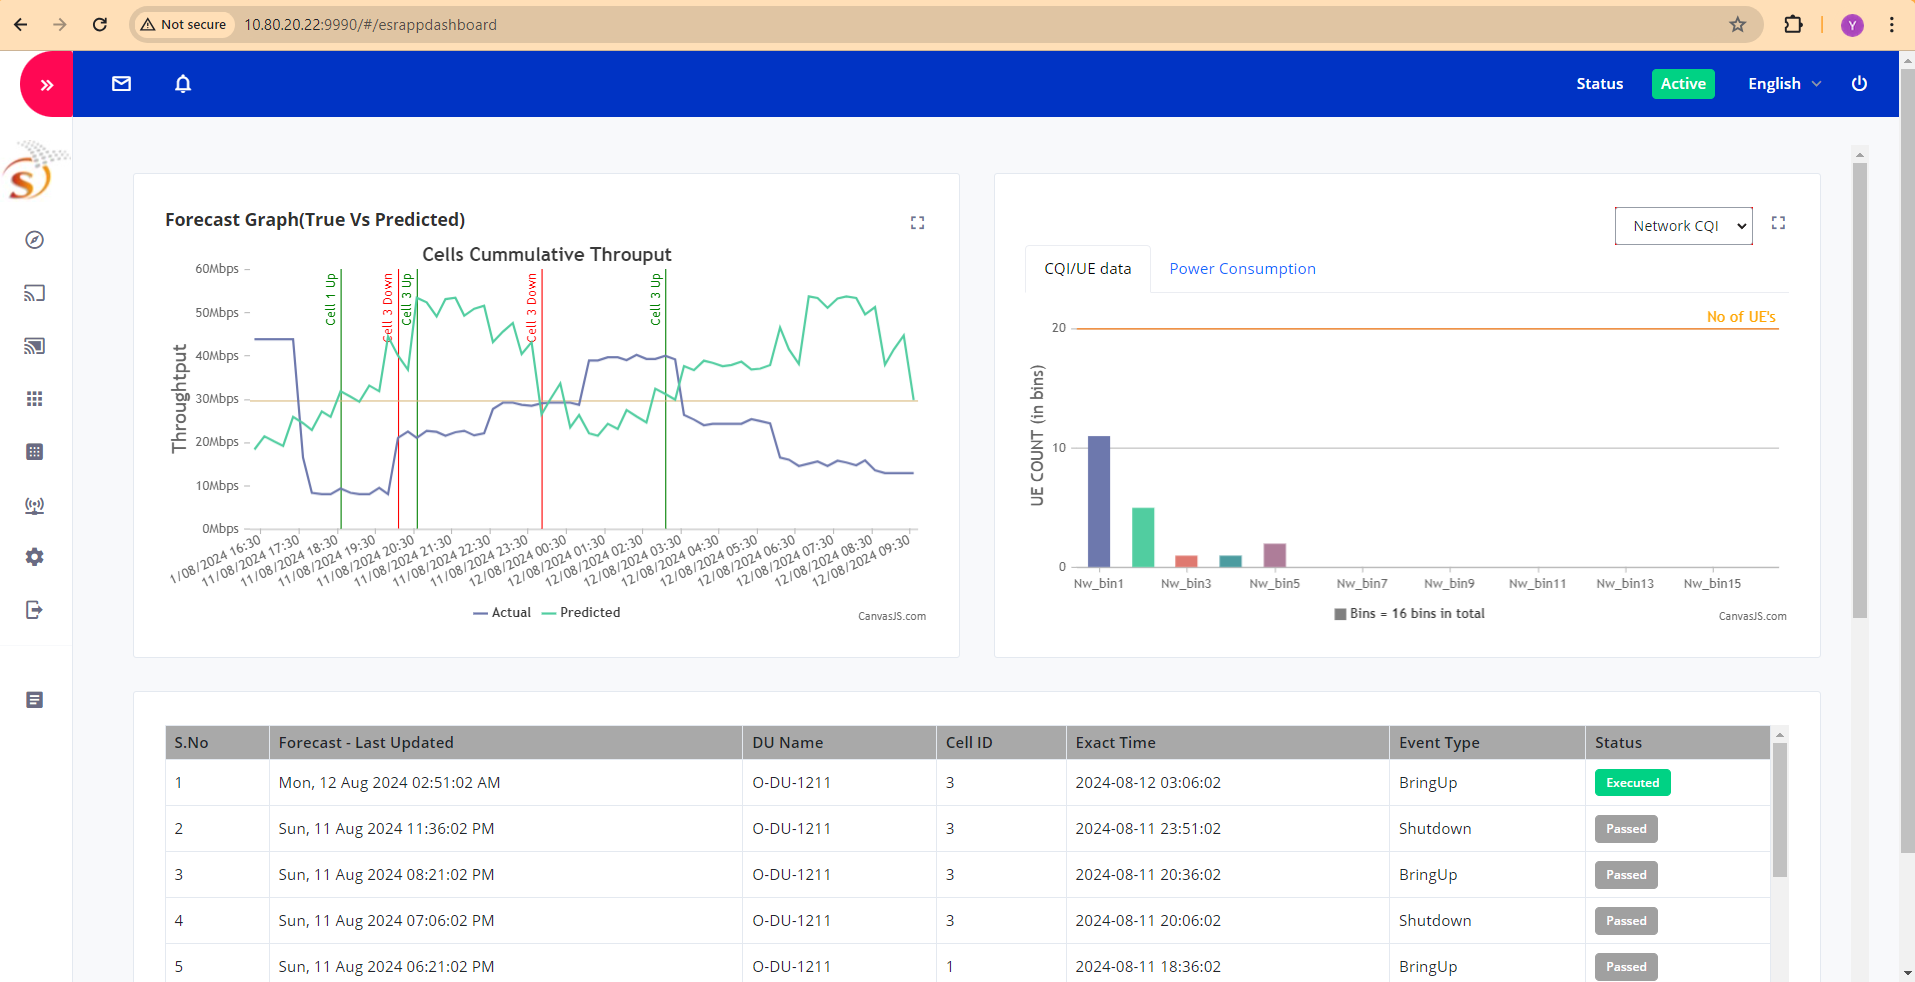
\includegraphics[width=0.5\textwidth]{/Users/pulakmehrotra/Desktop/SaankhyaLabs/es_oran_paper/acm_version_final/images/dashboard.png}
  \caption{ES rApp GUI}
  \label{fig:dashboard}
\end{figure}

\section{Design Rationale}
\label{sec:design_rationale}

In this section, we elucidate our reasoning behind the choice of regression model used to represent the overall network throughput.

\begin{comment}
\subsection{Decision Variables and Threshold Selection}

The decision-making process in any solution is governed by a set of decision variables that determine the course of action to be taken.
We proceed to evaluate the performance of our Energy Saving solution in terms of the three metrics mentioned below:
\begin{itemize}
  \item \textbf{Network CQI Distribution:} As described in [\textcolor{blue}{CITE}], we categorized the CQI values of the UEs based on the channel quality.
  \item \textbf{Network Throughput:} This metric represents the total throughput used by all the UEs connected to the system.
  \item \textbf{System Power Consumption:} This is the total power consumed by the system, measured in Watts (W).
\end{itemize}

The most important one to consider here is the throughput of the network, which is the primary metric used to decide whether a system needs a change in it's configiration or not.
The rationale behind this is simple: our focus is on the aggregate network performance, and throughput serves as a reliable metric for this purpose.
If the network state, specifically the channel quality and overall throughput, remains largely unchanged after the application of network-modifying policies, we deem the result acceptable.

The determination of thresholds for various decision variables is often crucial to the success of the algorithm. 
In this context, we aim to derive specific expressions to guide the selection of these variables.
In our proposed solutions, we have three primary decision variables: $\tau$, $\alpha_{th}$, and $P_{th}$.
- $\tau$ is the threshhold on the forecasted throughput, which is used to decide whether to shut down a cell or not.
- $\alpha_{th}$ is the allowed divergence of the forecasted/likely CQI distribution from the current CQI distribution. It is used to decide whether a policy should be implemented or not.
- $P_{th}$ is the threshold on the power consumption of the cell. Only cells function above a certain energy-consumption threshold are to be considered for shutdown/bringup.
\\
\textcolor{red}{[PRAMIT] \\
Could you please provide a short write-up on how $\tau$, $\alpha_{th}$ and $P_{th}$ are selected? What are the factors we consider?}
\end{comment}

\subsection{Datasets In Use}

We intended to find a regression model that, above all, identified the trend and seasonlity of traffic fluctuations.
The models underwent evaluation using a mix of four real-world and five synthetic time-series datasets, each exhibiting diverse trends and seasonal patterns:

\begin{itemize}
  \item Dataset 1: COMED Dataset - This real-world dataset, released by the Commonwealth Edison Company, illustrates the temporal variations in power consumption across a specific group of households.
  \item Dataset 2: Microsoft Dataset - This dataset, obtained using a data scraper, encapsulates the temporal variations in Microsoft's stock price.
  \item Dataset 3: Temperature Dataset - This dataset, sourced from Kaggle, depicts the temporal progression of the Earth's surface temperature.
  \item Dataset 4: No Trend Dataset - This synthetic dataset, created using a blend of sinusoidal and random noise functions, exhibits no discernible trend or seasonality.
  \item Dataset 5: Upwards Trend Dataset - This synthetic dataset is similar to Dataset 4, but it exhibits a noticeable upward trend (without any seasonality).
  \item Dataset 6: Downwards Trend Dataset - This synthetic dataset is similar to Dataset 4, but it exhibits a noticeable downward trend (without any seasonality).
  \item Dataset 7: Upwards Trend Dataset with Seasonality - Dataset 5 with added seasonality.
  \item Dataset 8: Downwards Trend Dataset with Seasonality - Dataset 6 with added seasonality.
  \item Dataset 9: Simulator Dataset - A synthetic dataset generated using our ns-3 simulator, taken to ensure that these models perform with traffic data and not just randomized time-serieses.
\end{itemize}

\subsection{Model Selection}
\begin{table*}[ht]
\caption{Performance of Different Models on Various Synthetic Datasets}
\centering
\resizebox{\textwidth}{!}{%
    \begin{tabular}{|*{3}{>{\centering\arraybackslash}p{0.33\textwidth}|}}
    \hline
    \textbf{Dataset Type} & \textbf{Prophet Performance} & \textbf{LSTM Performance} \\
    \hline
    No Trend, No Seasonality & Does not trend correctly, trends in the opposite direction & Follows trend but does not account for the noise well \\
    \hline
    Upwards Trend, No Seasonality & Steadily trends upwards but not according to the data (underfits) & Follows trend but predicts widely off values when accounting for noise \\
    \hline
    Downwards Trend, No Seasonality & Trends appropriately but underfits, does not recognize dataset intricacies & Recognizes trend and seasonality but produces very inaccurate values due to noise \\
    \hline
    Upwards Trend, With Seasonality & Recognizes trend but not seasonality & Recognizes trend and seasonality well, performs satisfactorily with test data \\
    \hline
    Downwards Trend, With Seasonality & Recognizes trend but not seasonality & Recognizes trend and seasonality but produces very inaccurate values due to noise \\
    \hline
    \end{tabular}%
}
\end{table*}

The choice of regression model used for Traffic Prediction is crucial to the success of the solution.
In this section, we compare the performance of three different regression models: Prophet, ARIMA, and LSTMs.
We train our models on all our real-world datasets (COMED, Microsoft and Temperature) and evaluate their performance on a validation set of the same dataset.
Our findings can be seen in \hyperref[tab:model_comp]{Table 1}.
We observe that the LSTM model outperforms Prophet, capturing the trend and seasonlity of the data the best.
The ARIMA model was found to be outright the worst performer, both taking the longest to train as well making forecasts completely ignoring the trend and seasonlity of the inputed data.
Considering how promising the LSTM's performance seemed, we decided to further evaluate the same.

\subsection{Model Verification}
\begin{table*}[ht]
    \caption{Performance of Different LSTM Models on Various Datasets}
    \centering
    \resizebox{\textwidth}{!}{%
      \begin{tabular}{|*{9}{>{\centering\arraybackslash}p{0.11\textwidth}|}}
        \hline
        \textbf{Dataset/Model} & \textbf{Model 1} & \textbf{Model 2} & \textbf{Model 3} & \textbf{Model 4} & \textbf{Model 5} & \textbf{Model 6} & \textbf{Model 7} & \textbf{Model 8} \\
        \hline
        \textbf{Model 1} & 0.044 & 0.0054 & 0.2507 & 2.0302 & 0.6256 & 1.8354 & 1.186 & 1.1158 \\
        \hline
        \textbf{Model 2} & 0.3358 & 0.2262 & 0.2609 & 0.915 & 0.2613 & 0.855 & 0.486 & 0.4774 \\
        \hline
        \textbf{Model 3} & 0.5695 & 0.7270 & 0.4274 & 1.0624 & 0.3611 & 1.091 & 0.6027 & 0.593 \\
        \hline
        \textbf{Model 4} & 1.0267 & 0.5424 & 0.7875 & 0.5457 & 0.7711 & 1.3335 & 0.6144 & 0.9841 \\
        \hline
        \textbf{Model 5} & 0.5713 & 0.6027 & 0.4731 & 1.069 & 0.2857 & 1.011 & 0.5556 & 0.5418 \\
        \hline
        \textbf{Model 6} & 1.3595 & 1.1141 & 1.3407 & 1.2204 & 0.9841 & 1.2831 & 1.0261 & 1.0280 \\
        \hline
        \textbf{Model 7} & 0.5459 & 0.3503 & 0.2500 & 0.9837 & 0.2005 & 0.9108 & 0.4610 & 0.4590 \\
        \hline
        \textbf{Model 8} & 0.5806 & 0.2504 & 0.1865 & 0.9605 & 0.1640 & 0.8965 & 0.417 & 0.4134 \\
        \hline
      \end{tabular}%
    }
  \end{table*}
  
  

After arriving at using LSTMs as the model of choice for traffic forecasting, we had to ensure that the model would be able to handle the simulated load. 
We did so using synthetic data of various types, as outlined in our Dataset section.
To verify the robustness of the model's forecasts, we trained the LSTM models using a diverse range of datasets, each exhibiting unique general trends.
For each dataset, we trained a corresponding LSTM model. 
We used Mean Squared Error (MSE) as an evaluation index to evaluate the forecast accuracy of the models.
Subsequently, we cross-validated each trained model with the remaining datasets.
The MSE values of all the trained models and the datasets in use is described in in \hyperref[tab:lstm_performance]{Table 2}.
We observe that the LSTM trained on data with more seasonlity (model 7,8 and 9) perform the best all around, with the lowest MSE values.
This is expected, as the LSTM model is designed to capture the long-term dependencies in the data, which are more prevalent in datasets with seasonality.
  
Therefore, when training our model on real-world data, we should ensure that the data has a significant amount of seasonality to ensure the best performance.  
The amount of data used to train the LSTM model is crucial to the success of the solution.
If we train the model on excessive data, the model may overfit to the training data and fail to generalize to unseen data.
This would be especially catastrophic in our specific use case, as we
This will depend on the deployemnt environment's complexity, and in our specific setup we found 300 samples to suffice.

